\begin{figure}[ht]
    \centering
    %\begin{adjustbox}{width=0.8\linewidth}
    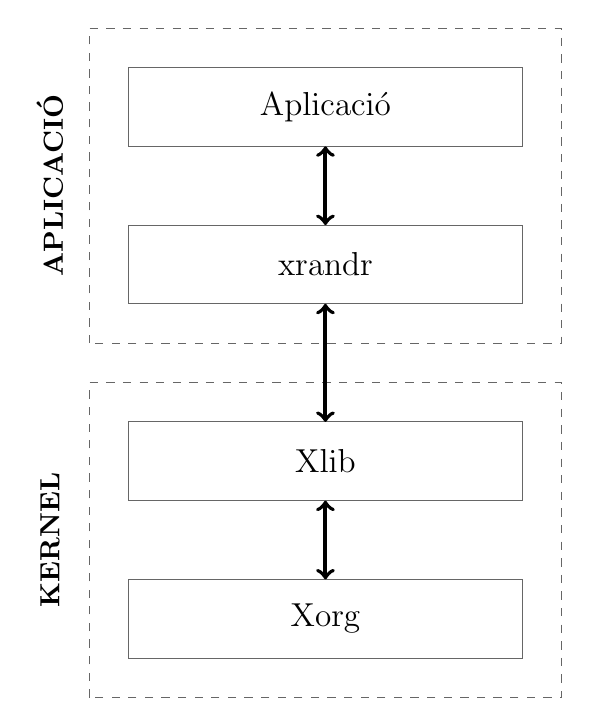
\begin{tikzpicture}

        \filldraw[fill=white, draw=black!60!white,dashed] (0.5,0) rectangle (6.5,4);
        \filldraw[fill=white, draw=black!60!white,dashed] (0.5,4.5) rectangle (6.5,8.5);

    
        \filldraw[fill=white, draw=black!60!white] (1,0.5) rectangle (6,1.5);
        \filldraw[fill=white, draw=black!60!white] (1,2.5) rectangle (6,3.5);

        \filldraw[fill=white, draw=black!60!white] (1,5) rectangle (6,6);
        \filldraw[fill=white, draw=black!60!white] (1,7) rectangle (6,8);

        \node at (3.5,1) {\large Xorg};
        \node at (3.5,3) {\large Xlib};
        \node at (3.5,5.5) {\large xrandr};
        \node at (3.5,7.5) {\large Aplicació};

        \node at (0,2) {\rotatebox{90}{\textbf{KERNEL}}};
        \node at (0,6.5) {\rotatebox{90}{\textbf{APLICACIÓ}}};

        \draw[line width=0.5mm, <->] (3.5,1.5) -- (3.5,2.5);
        \draw[line width=0.5mm, <->] (3.5,3.5) -- (3.5,5);
        \draw[line width=0.5mm, <->] (3.5,6) -- (3.5,7);

    \end{tikzpicture}
    %\end{adjustbox}

    \caption{Intermediaris entre \est{Xorg} i l'aplicació final \cite{Xrandr}.}
    \label{fig:xorg-hyerarchy}
\end{figure}
